%
%                  Politecnico di Milano
%
%         Student: Caravano Andrea, Alberto Cantele
%            A.Y.: 2024/2025
%
%   Last modified: 05/04/2025
%
%     Description: Internet of Things: Challenge n. 2
%                  Theoretical exercise
%

\documentclass[a4paper,11pt]{article} % tipo di documento
\usepackage[T1]{fontenc} % codifica dei font
\usepackage[utf8]{inputenc} % lettere accentate da tastiera
\usepackage[english]{babel} % lingua del documento
\usepackage{lipsum} % genera testo fittizio
\usepackage{url} % per scrivere gli indirizzi Internet e/o di riferimento nella pagina

\usepackage[hidelinks]{hyperref} % per modificare il comportamento dei collegamenti ipertestuali (+ leva colore attorno)

\usepackage[margin=0.7in]{geometry} % margine di pagina

\usepackage{graphicx} % per inserire immagini

\usepackage[outputdir=../auxil]{minted} % per colorazione automatica del codice (installare pygments da Homebrew)
% \usepackage{pythonhighlight} % per Python

\setminted{ % si può impostare il linguaggio specifico con \setminted[JSON] ad esempio
    linenos=true,
    breaklines=true,
    encoding=utf8,
    fontsize=\normalsize,
    frame=lines
}

\usepackage{fancyhdr}
\usepackage{textcomp}
\usepackage{siunitx} % per gestione intestazione e piè di pagina

\usepackage{tcolorbox} % per riquadrature di vario colore

\usepackage{float} % per figure comparative flottanti
\usepackage{amsmath} % per frazioni in display style

\usepackage{icomma} % virgola come separatore decimale

\usepackage{titlesec} % per configurazione del tipo paragrafo

% setup del tipo paragrafo
\setcounter{secnumdepth}{4}

\titleformat{\paragraph}
{\normalfont\normalsize\bfseries}{\theparagraph}{1em}{}
\titlespacing*{\paragraph}
{0pt}{3.25ex plus 1ex minus .2ex}{1.5ex plus .2ex}

\hypersetup{ % metadati di titolo e autore nel PDF
    pdftitle={Internet of Things: Challenge n. 2},
    pdfauthor={Andrea Caravano, Alberto Cantele}
}

\setlength{\parindent}{0pt} % rimuove l'indentazione del testo

\tcbset{ % impostazioni per riquadrature
    colback=gray!20,
    colframe=black,
    boxrule=0.5pt
}

\begin{document}
    \pagestyle{fancy}
    \fancyhead{}\fancyfoot{}
    \fancyhead[L]{\textbf{Internet of Things: Challenge n. 2}}
    \fancyhead[R]{Andrea Caravano, Alberto Cantele}
    \fancyfoot[C]{\thepage}

    \title{\textbf{Internet of Things}\\Challenge n. 2: Theoretical exercise}
    \author{Andrea Caravano, Alberto Cantele}
    \date{Academic Year 2024--25}
    \maketitle

    \tableofcontents

    \newpage


    \section{Exercise text}\label{sec:exercise-text}
    A wireless IoT network consists of the following devices:

    \begin{itemize}
        \item A battery-powered, Wi-Fi-enabled \textbf{temperature sensor} that measures and transmits temperature data every 5 minutes.
        \item A battery-powered, Wi-Fi-enabled \textbf{valve} that receives temperature readings from the sensor and computes the average temperature every 30 minutes to decide whether to open or close.
        \item \textbf{A Raspberry Pi}, connected to the power grid, which only supports MQTT for communication.
    \end{itemize}

    The temperature sensor and valve can communicate using either \textbf{MQTT} or \textbf{CoAP}, with a specific pre-defined topic or resource.
    The topic/resource length is 10 bytes and the payload size is 8 bytes.
    However, since the Raspberry Pi only supports MQTT, any interaction between the Raspberry Pi and the battery-operated devices must use MQTT.
    The sensor and valve, however, can communicate directly using CoAP if desired.

    Consider the following message sizes (in bytes), which \textbf{already include} header and payload size for the COAP resource or MQTT topic used in the system:

    \label{message-sizes-table}

    \begin{center}
        \begin{tabular}{|c|c|c|c|}
            \hline
            \multicolumn{2}{|c|}{CoAP} & \multicolumn{2}{|c|}{MQTT} \\
            \hline
            GET Request  & 60 B & Subscribe     & 58 B \\
            \hline
            GET Response & 55 B & Sub Ack       & 52 B \\
            \hline
            PUT Request  & 77 B & Publish       & 68 B \\
            \hline
            PUT Response & 58 B & Pub Ack       & 51 B \\
            \hline
            Empty ACK    & 14 B & Connect       & 54 B \\
            \hline
            &      & Connect ACK   & 47 B \\
            \hline
            &      & Ping Request  & 52 B \\
            \hline
            &      & Ping Response & 48 B \\
            \hline
        \end{tabular}
    \end{center}

    \textbf{Assuming that:}

    \begin{enumerate}
        \item Transmit and Receive cost per bit are:

        \textbf{$E_{TX} = 50$ nJ/bit, $E_{RX} = 58$ nJ/bit (nanojoule per bit)}
        \item The Wi-Fi network is ideal \textbf{(no losses)}
        \item The processing cost on the valve to compute the average temperature every 30 minutes is \textbf{$E_c = 2.4$ mJ (millijoule)}
        \item The sensor and valve start in power-off state
    \end{enumerate}

    \textbf{Exercise Question 1 (EQ1)}: Compute the total energy consumed by the two battery-powered devices \textbf{over a period of 24 hours} in both cases when using COAP \textbf{(a)} and MQTT \textbf{(b)}, using each in its \textbf{most efficient configuration energy-wise}.

    \medskip

    \textbf{Exercise Question 2 (EQ2)}: Propose \textbf{at least one} solution for decreasing the energy consumption when passing using the Raspberry PI as a broker.
    \textbf{Give a rough estimate of the energy saving} that could be obtained with your solution: recompute the energy under your proposed configuration.

    \medskip

    Let's tackle each point singularly.


    \section{A 24-hour complete cycle, from power-off}\label{sec:a-24-hour-complete-cycle-from-power-off}

    \subsection{CoAP}\label{subsec:coap}

    \subsubsection{The most efficient configuration energy-wise}

    Of course, in this point of the exercise, we are assuming to follow slavishly all the details of the protocol definition.

    The most reasonably energy-efficient configuration that uses CoAP as an application-layer communication protocol is the one mimicking a Publish-Subscribe communication style, through the observe pattern.

    For resources that allow observation, a CoAP client just needs to specify an additional option to the \textsc{GET Request} message, registering for reception of all the updates to the interested resource.

    The next point to consider is \textsc{CONfirmable} or \textsc{NON-confirmable} messages: the first kind provide stronger guarantees, being them shifted to the application layer for CoAP, but does not perform well, energy-wise.

    Instead, \textsc{NON-confirmable} messages only require an initial request, serving as a registration for the observable object.
    Then, any successive value will come as a \textsc{Response}, without requiring an \textsc{ACK} from the Client.

    A comparison among the two is shown in the following test environment.

    \begin{figure}[H]
        \centering
        \subfloat{{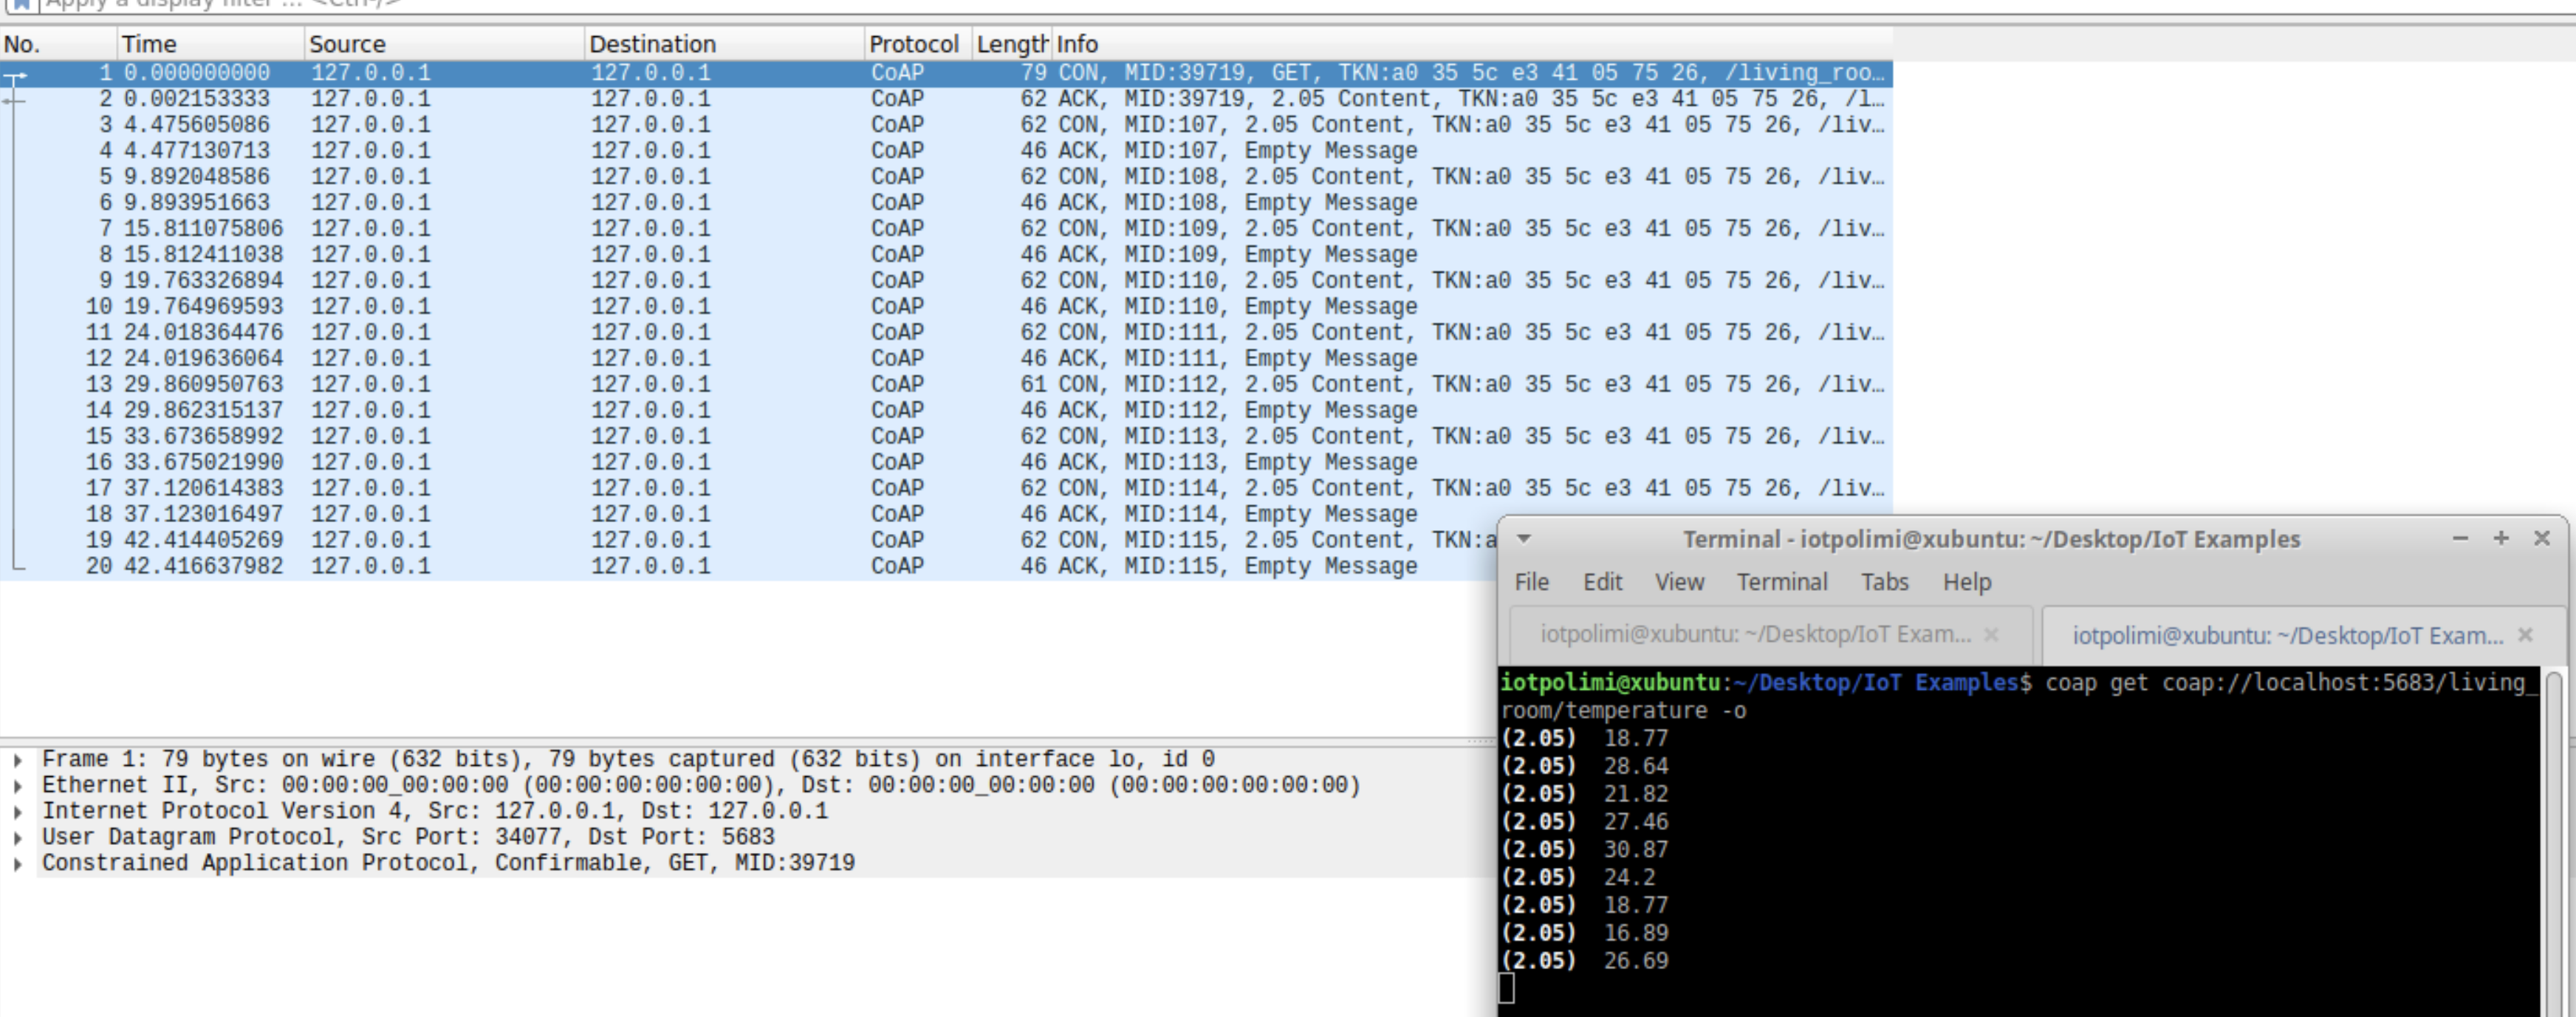
\includegraphics[width=14.0cm]{../res/CoAP-CON-case} }}
        \qquad
        \subfloat{{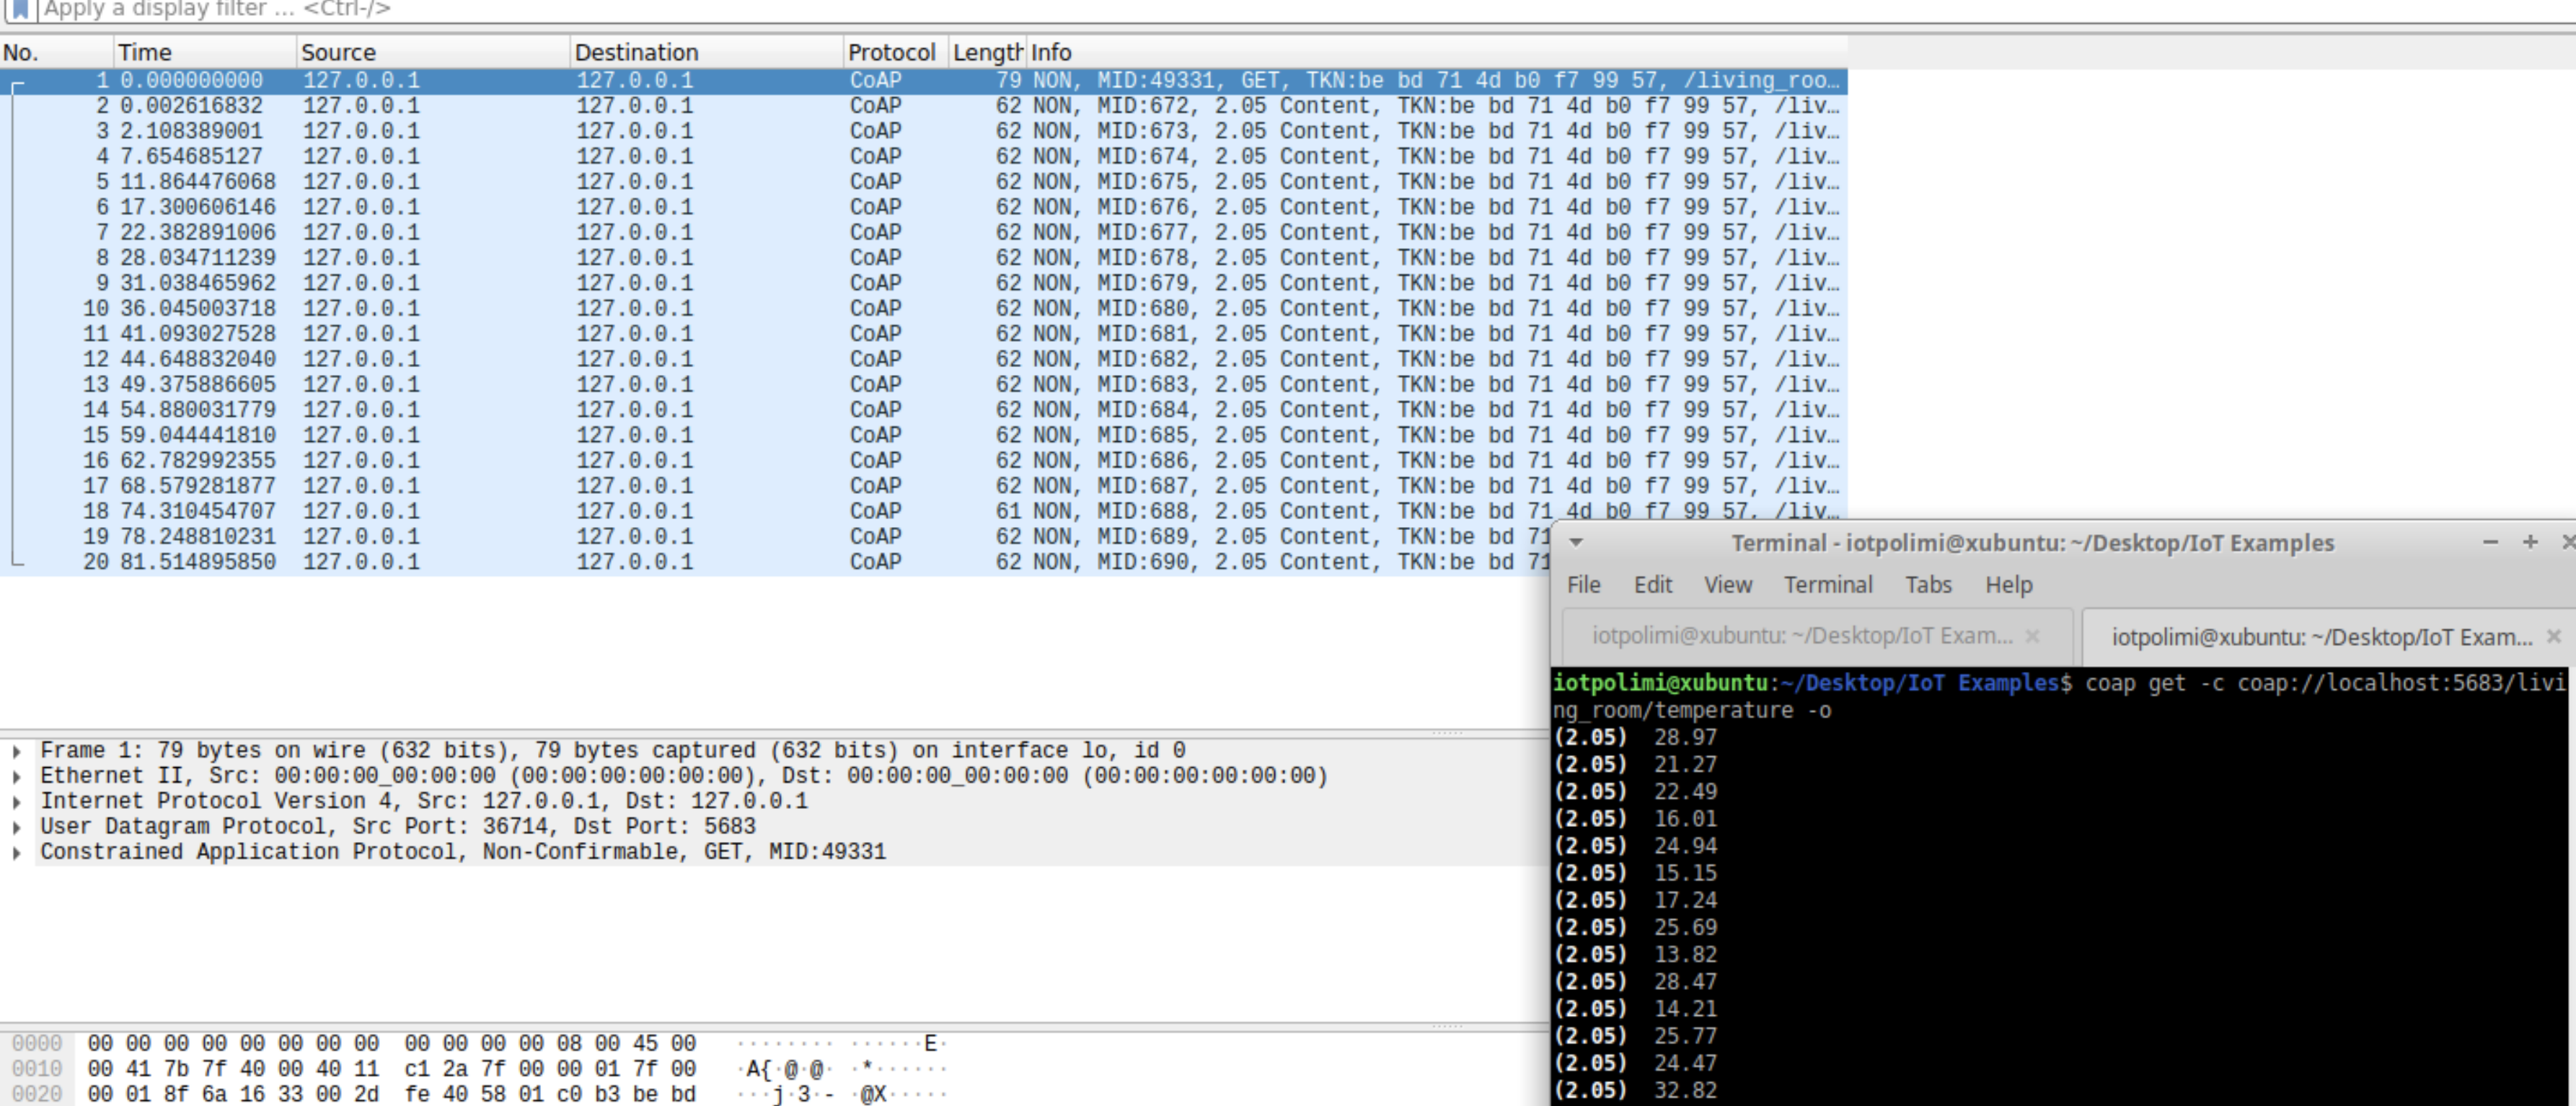
\includegraphics[width=14.0cm]{../res/CoAP-NON-case} }}
        \caption{Comparison: \textsc{CONfirmable} messages versus \textsc{NON-confirmable} messages}
        \label{fig:comparison-coap}
    \end{figure}

    \subsubsection{Communication diagram}

    The resulting communication diagram is shown in the following.
    Please note that the propagation time, in this case, is not interesting during the calculation steps.

    \begin{center}
        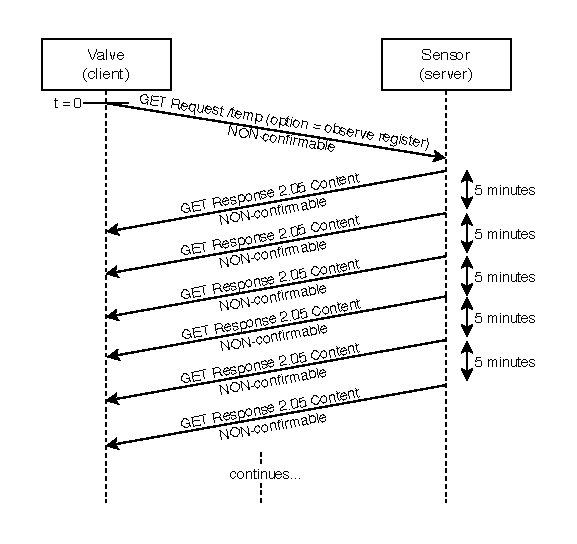
\includegraphics[width=13cm]{../res/communication-diagram-coap}
    \end{center}

    \subsubsection{Solution scheme}

    Data declaration:

    \medskip

    Given the \hyperref[message-sizes-table]{message sizes as part of the text},

    \smallskip

    Energy spent for transmission ($E_{TX}$)$\ = 50$ nJ/bit,

    \smallskip

    Energy spent for reception ($E_{RX}$)$\ = 58$ nJ/bit,

    \smallskip

    Energy spent for average computation at the valve ($E_c$)$\ = 2,4$ mJ,

    \smallskip

    Being $L_{GET\ Request}$ and $L_{GET\ Response}$ the message sizes for the \textsc{GET Request} (including the option to register for observation) and \textsc{GET Response} packets (carrying the temperature data), respectively.

    \bigskip

    We are able to compute the number of bytes transmitted and received by each battery-operated node and therefore the energy consumed, overall.

    \paragraph{Sensor}

    $L_{SENSOR, TX} = \dfrac{24 \cdot 60\ minutes}{5\ minutes} \cdot L_{GET\ Response} = 288 \cdot 55$ bytes $ = 15840$ bytes

    \medskip

    With the fraction representing the frequency of temperature updates sent via a \textsc{GET Response} (every 5 minutes, 12 per hour).

    \smallskip

    $L_{SENSOR, RX} = 1 \cdot L_{GET\ Request} = 60$ bytes

    \paragraph{Valve}

    $L_{VALVE, TX} = 1 \cdot L_{GET\ Request} = 60$ bytes

    \medskip

    $L_{VALVE, RX} = \dfrac{24 \cdot 60\ minutes}{5\ minutes} \cdot L_{GET\ Response} = 288 \cdot 55$ bytes $ = 15840$ bytes

    \paragraph{Energy computation}

    Let's define

    \bigskip

    $E_{TX} = \dfrac{50\ nJ}{1\ bit} = \dfrac{400\ nJ}{1\ byte = 1\ bit \cdot 8}$

    \medskip

    $E_{RX} = \dfrac{58\ nJ}{1\ bit} = \dfrac{464\ nJ}{1\ byte = 1\ bit \cdot 8}$

    \medskip

    $E_{c \ per \ day} = 2,4\ mJ \cdot \dfrac{24 \cdot 60\ minutes}{30\ minutes} = 115,200$ mJ

    \bigskip

    Being a byte composed by 8 bits

    \smallskip

    Then, we have that, finally:

    \medskip

    $E_{SENSOR} = E_{TX} \cdot L_{SENSOR, TX} + E_{RX} \cdot L_{SENSOR, RX} = 15840\ bytes \, \cdot 400\ nJ/byte + 60\ bytes \, \cdot 464\ nJ/byte = 6,336\ mJ\ + 27,840\ \mu J = 6,364\ mJ$

    \medskip

    $E_{VALVE} = E_{TX} \cdot L_{VALVE, TX} + E_{RX} \cdot L_{VALVE, RX} + E_{c \ per \ day} = 60\ bytes \, \cdot 400\ nJ/byte + 15840\ bytes \, \cdot 464\ nJ/byte + 115,200\ mJ = 24,000\ \mu J + 7,350\ mJ + 115,200\ mJ = 122,574\ mJ$

    \medskip

    $E_{TOTAL} = E_{SENSOR} + E_{VALVE} = 6,364\ mJ + 122,574\ mJ = 128,938\ mJ$

    \subsection{MQTT}\label{subsec:mqtt}

    \subsubsection{The most efficient configuration energy-wise}

    Of course, in this point of the exercise, we are assuming to follow slavishly all the details of the protocol definition.

    The most relevant energy-consuming element of the protocol can definitely be located in the overhead coming from both reliability at transport and application layer.

    The transport protocol (TCP) is not something which can be moved away from the architecture, but the Quality of Service level at the application layer can instead be minimized, therefore minimizing energy consumption.

    This behaviour can be achieved by using the QoS level 0.

    Note, however, that, independently of the chosen reliability level, a \textsc{CONNECT} message will have its matching \textsc{CONNECT ACK} and each \textsc{SUBSCRIBE} will have its own \textsc{SUBSCRIBE ACK}.

    Other kinds of messages require an acknowledgement from the broker, like the \textsc{UNSUBSCRIBE} one, reporting back with the status code for each subscription.

    In our case, these last are not interesting.

    Let's now simulate the system publishing a few simulated temperature measurements.

    \begin{figure}[H]
        \centering
        \subfloat{{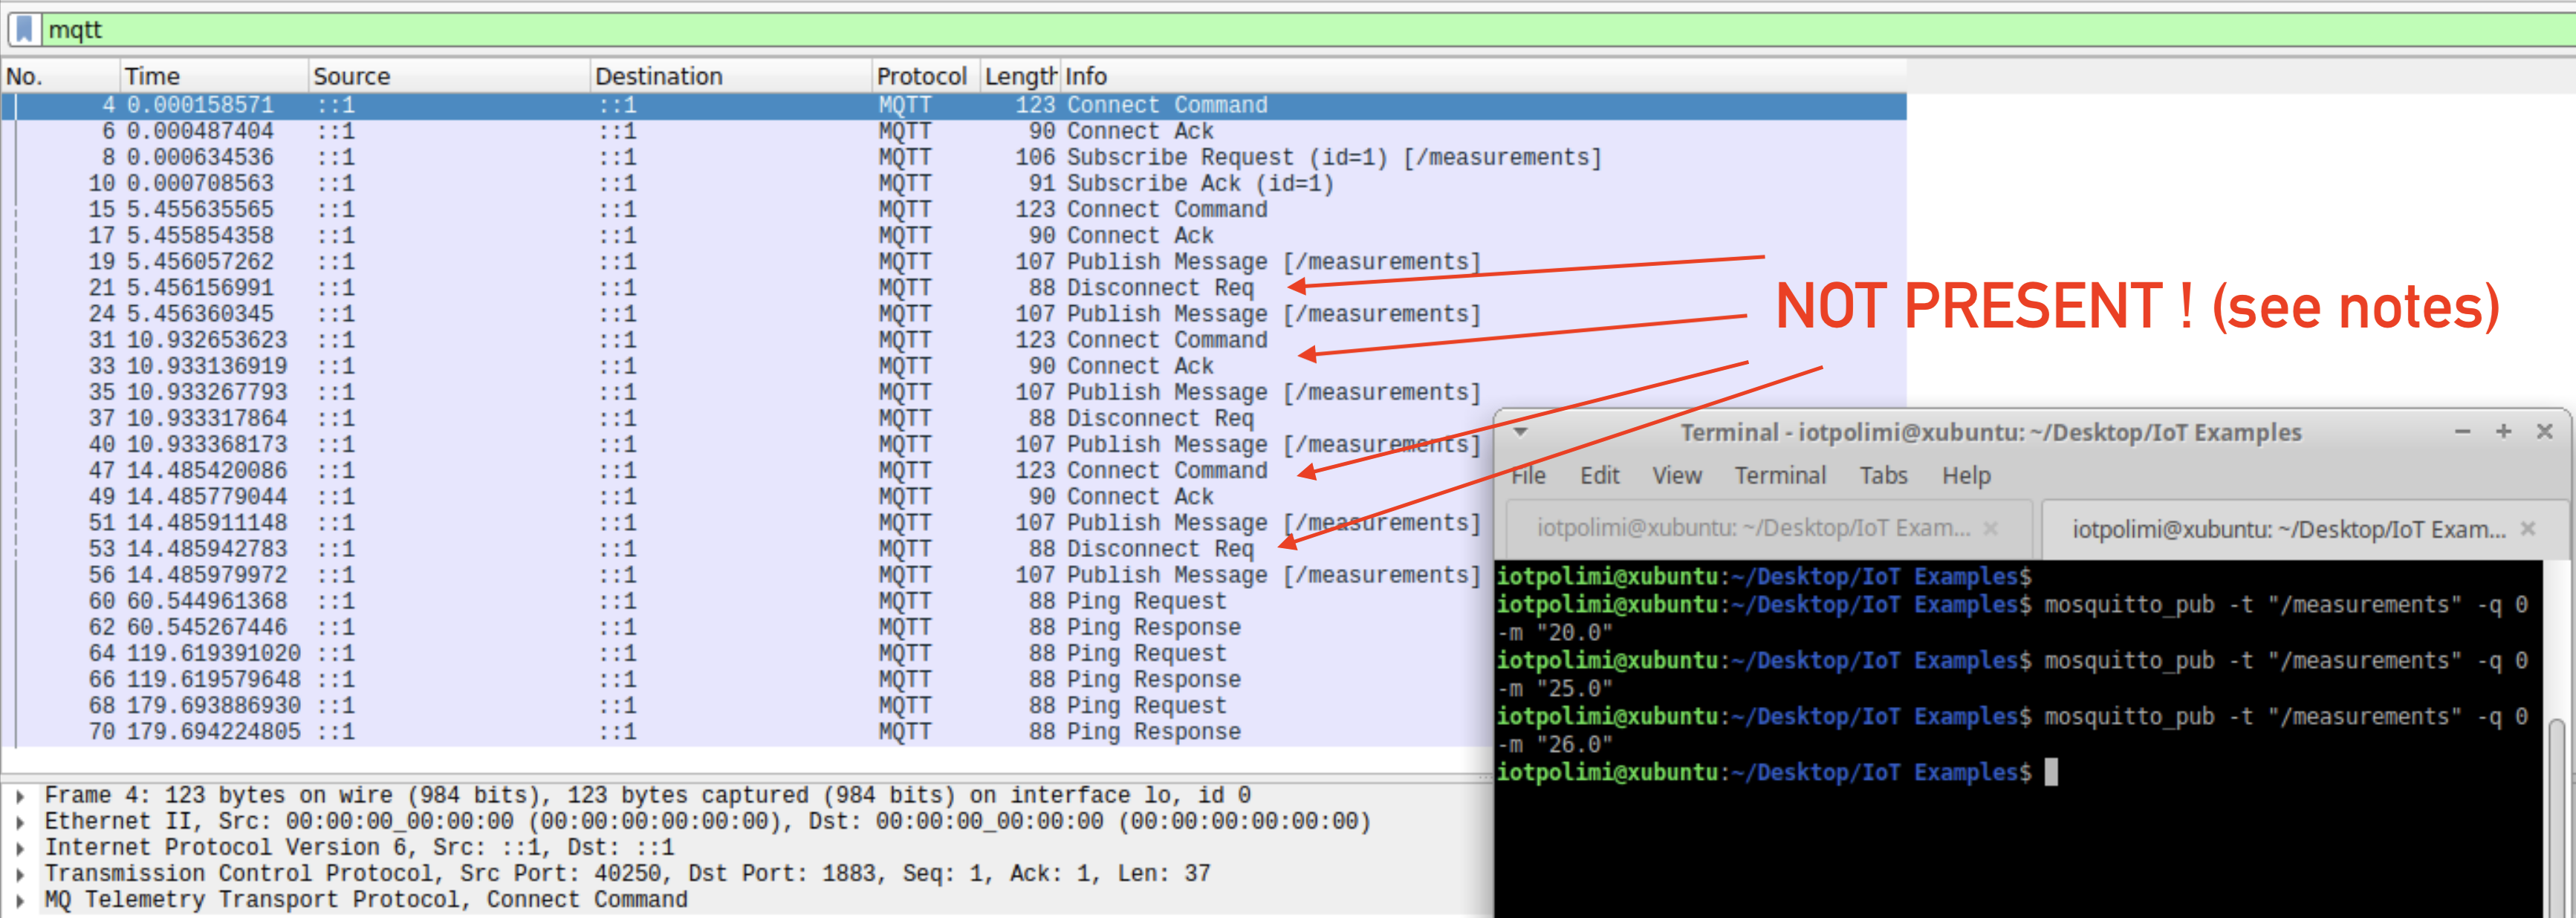
\includegraphics[width=16.5cm]{../res/Example-MQTT-note} }}
        \caption{A simulation of the system}
        \label{fig:mqtt-wireshark}
    \end{figure}

    \label{liveness-mqtt}

    In our description, we have still not mentioned the liveness properties of the system: both subscribers and publishers keep an active session with the broker for the whole time?
    Moreover, are there any liveness timeouts (keep-alives)?

    \smallskip

    To address the first one, it is important to note that each choice is implementation dependent and no actual protocol requirements impose a certain session duration limit.

    However, since we are operating in the field of IoT and no other MQTT messages are expected other than the periodic \textsc{PUBLISH} updates, a reasonable choice is to \textbf{keep the session open while the device is on}.

    Closing it at each \textsc{PUBLISH} message from the sensor side, in fact, requires, from our exterior understanding of the system, more energy than persisting a state of the session in the internal device memory (3 more messages would be required at every update of the temperature: a \textsc{DISCONNECT} message and a pair of \textsc{CONNECT} and \textsc{CONNECT ACK} being respectfully sent and received).

    \smallskip

    No processing power is needed, instead, while data transmission/reception is not ongoing.

    \smallskip

    A special exception are liveness timeouts, that instead requires radio operation and are, in fact, added to the final energy term: they are implemented through keep-alives, being composed of the pair of \textsc{PING REQUEST} and \textsc{PING RESPONSE} messages.

    How frequent is the pair of \textsc{PING REQUEST} and \textsc{PING RESPONSE} messages?
    Again, the protocol does not impose a strict upper or lower bound to the frequency of keep-alives, which are instead left to the implementation.

    Since, for our laboratory activities, \textsc{Mosquitto} is the \textbf{reference implementation, the assumed default for liveness timeouts is 60 seconds (1 minute)}.

    A very reasonable optimization choice would require the removal of liveness constraints completely, acting on the specific implementation parameters, rather than the protocol itself.

    The \hyperref[subsubsec:deletion-liveness]{first optimization proposal}, in fact, builds exactly on this intuition.

    \subsubsection{Communication diagram}

    The resulting communication diagram is shown in the following.
    Please note that the propagation time, in this case, is not interesting during the calculation steps.

    \begin{center}
        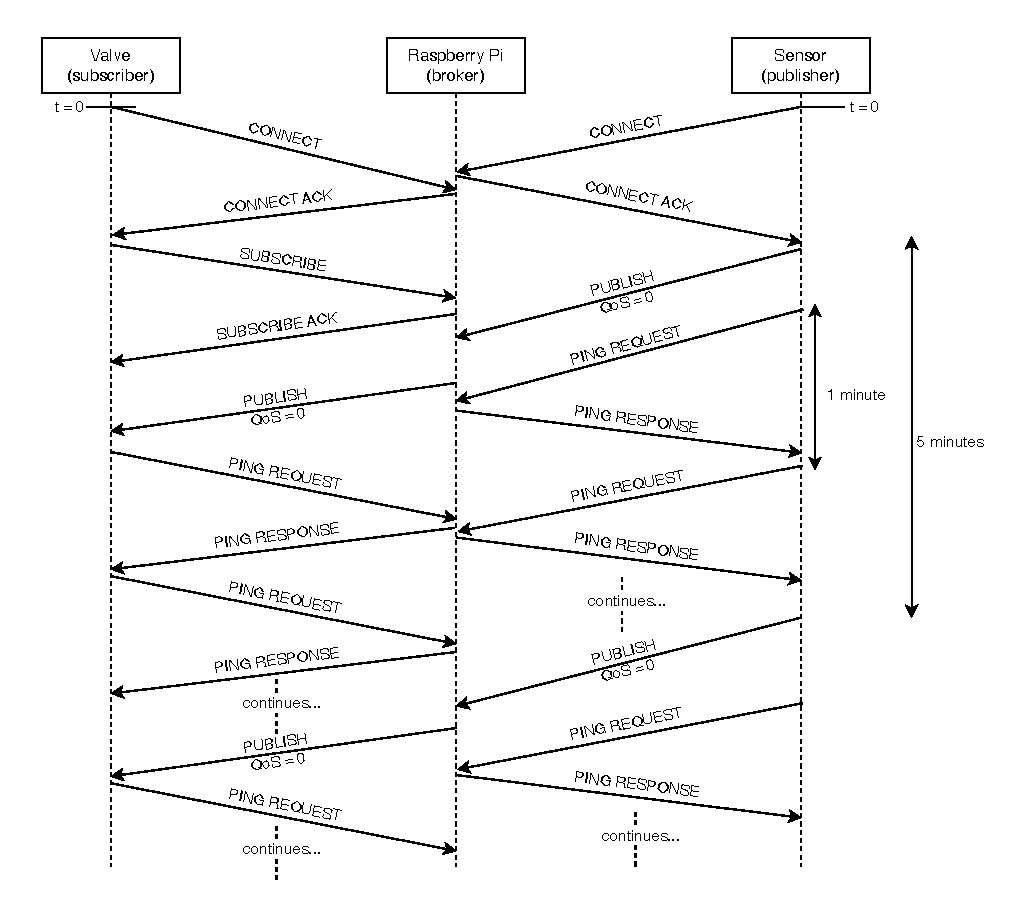
\includegraphics[width=13cm]{../res/communication-diagram-mqtt}
    \end{center}

    \subsubsection{Solution scheme}

    Data declaration:

    \medskip

    Given the \hyperref[message-sizes-table]{message sizes as part of the text},

    \smallskip

    Energy spent for transmission ($E_{TX}$)$\ = 50$ nJ/bit,

    \smallskip

    Energy spent for reception ($E_{RX}$)$\ = 58$ nJ/bit,

    \smallskip

    Energy spent for average computation at the valve ($E_c$)$\ = 2,4$ mJ,

    \smallskip

    Being $L_{CONN}$, $L_{CONNACK}$, $L_{SUB}$, $L_{SUBACK}$, $L_{PUB}$, $L_{PINGREQ}$, $L_{PINGRESP}$ the message sizes for the \textsc{CONNECT}, \textsc{CONNECT ACK}, \textsc{SUBSCRIBE}, \textsc{SUBSCRIBE ACK}, \textsc{PUBLISH}, \textsc{PING REQUEST}, \textsc{PING RESPONSE} message types, respectively.

    \bigskip

    We are able to compute the number of bytes transmitted and received by each battery-operated node and therefore the energy consumed, overall.

    \paragraph{Sensor}

    $L_{SENSOR, TX} = 1 \cdot L_{CONN} + \dfrac{24 \cdot 60\ minutes}{5\ minutes} \cdot L_{PUB} + \dfrac{24 \cdot 60\ minutes}{1\ minute} \cdot L_{PINGREQ}$

    \medskip

    \qquad \qquad \qquad $ = 54$ bytes $+\ 288 \cdot 68$ bytes $+\ 1440 \cdot 52$ bytes $ = 94518$ bytes

    \medskip

    With the fraction representing the frequency of temperature updates sent via a \textsc{PUBLISH} message (every 5 minutes, 12 per hour) and frequency of the \textsc{PING REQUEST} message (liveness timeout).

    \medskip

    $L_{SENSOR, RX} = 1 \cdot L_{CONNACK} + \dfrac{24 \cdot 60\ minutes}{1\ minute} \cdot L_{PINGRESP}$

    \medskip

    \qquad \qquad \qquad $= 47$ bytes $+\ 1440 \cdot 48$ bytes $ = 69167$ bytes

    \paragraph{Valve}

    $L_{VALVE, TX} = 1 \cdot L_{CONN} + 1 \cdot L_{SUB} + \dfrac{24 \cdot 60\ minutes}{1\ minute} \cdot L_{PINGREQ}$

    \medskip

    \qquad \qquad \qquad $= 54$ bytes $+\ 58$ bytes $+\ 1440 \cdot 52$ bytes $ = 74992$ bytes

    \medskip

    $L_{VALVE, RX} = 1 \cdot L_{CONNACK} + 1 \cdot L_{SUBACK} + \dfrac{24 \cdot 60\ minutes}{5\ minutes} \cdot L_{PUB} + \dfrac{24 \cdot 60\ minutes}{1\ minute} \cdot L_{PINGRESP}$

    \medskip

    \qquad \qquad \qquad $= 47$ bytes $+\ 52$ bytes $+\ 288 \cdot 68$ bytes $+\ 1440 \cdot 48$ bytes $= 88803$ bytes

    \paragraph{Energy computation}

    Let's define

    \bigskip

    $E_{TX} = \dfrac{50\ nJ}{1\ bit} = \dfrac{400\ nJ}{1\ byte = 1\ bit \cdot 8}$

    \medskip

    $E_{RX} = \dfrac{58\ nJ}{1\ bit} = \dfrac{464\ nJ}{1\ byte = 1\ bit \cdot 8}$

    \medskip

    $E_{c \ per \ day} = 2,4\ mJ \cdot \dfrac{24 \cdot 60\ minutes}{30\ minutes} = 115,2$ mJ

    \bigskip

    Being a byte composed by 8 bits

    \smallskip

    Then, we have that, finally:

    \medskip

    $E_{SENSOR} = E_{TX} \cdot L_{SENSOR, TX} + E_{RX} \cdot L_{SENSOR, RX} = 94518\ bytes \, \cdot 400\ nJ/byte + 69167\ bytes \, \cdot 464\ nJ/byte = 37,807\ mJ\ + 32,093\ mJ = 69,900\ mJ$

    \medskip

    $E_{VALVE} = E_{TX} \cdot L_{VALVE, TX} + E_{RX} \cdot L_{VALVE, RX} + E_{c \ per \ day} = 74992\ bytes \, \cdot 400\ nJ/byte + 88803\ bytes \, \cdot 464\ nJ/byte + 115,200\ mJ = 30,000\ mJ + 41,205\ mJ + 115,200\ mJ = 186,404\ mJ$

    \medskip

    $E_{TOTAL} = E_{SENSOR} + E_{VALVE} = 69,900\ mJ + 186,404\ mJ = 256,304\ mJ$


    \section{Improvements proposals and possible revisions}\label{sec:improvements-proposals-and-possible-revisions}
    The main point of leverage for optimizations focuses on message exchange and temperature averaging computation, being, of course, the most energy-relevant elements for the system.

    The frequency and kind of messages exchanged among the nodes are the main point to tackle, alongside computational capabilities, when reviewing the overall structure of the communication.

    \subsection{MQTT}
    The following proposals aim at minimizing the number of messages exchanged between different battery-operated nodes.
    They will also include some restructurization of the network schema to fully explore the range of possibilities to still solve the problem, but more efficiently.

    \subsubsection{Deletion of the liveness constraints}
    \label{subsubsec:deletion-liveness}

    \hyperref[liveness-mqtt]{As mentioned in the beginning}, there is no specific upper or lower bound to the liveness constraints dictated by the protocol (that implements it through the pair of \textsc{PING REQUEST} and \textsc{PING RESPONSE} messages), but it's mainly left to the specific implementation.

    As we are operating in an IoT scenario, the complete removal of the liveness constraint will definitely provide a huge benefit to the overall energy consumption.

    \smallskip

    Let's explore this possibility:

    \medskip

    \paragraph{Sensor}

    $L_{SENSOR, TX} = 1 \cdot L_{CONN} + \dfrac{24 \cdot 60\ minutes}{5\ minutes} \cdot L_{PUB} = 54$ bytes $+\ 288 \cdot 68$ bytes $ = 19638$ bytes

    \medskip

    $L_{SENSOR, RX} = 1 \cdot L_{CONNACK} = 47$ bytes

    \paragraph{Valve}

    $L_{VALVE, TX} = 1 \cdot L_{CONN} + 1 \cdot L_{SUB} = 54$ bytes $+\ 58$ bytes $ = 112$ bytes

    \medskip

    $L_{VALVE, RX} = 1 \cdot L_{CONNACK} + 1 \cdot L_{SUBACK} + \dfrac{24 \cdot 60\ minutes}{5\ minutes} \cdot L_{PUB}$

    \medskip

    \qquad \qquad \qquad $= 47$ bytes $+\ 52$ bytes $+\ 288 \cdot 68$ bytes $= 19683$ bytes

    \paragraph{Energy computation}

    $E_{SENSOR} = E_{TX} \cdot L_{SENSOR, TX} + E_{RX} \cdot L_{SENSOR, RX} = 19638\ bytes \, \cdot 400\ nJ/byte + 47\ bytes \, \cdot 464\ nJ/byte = 7,855\ mJ\ + 21,808\ \mu J = 7,877\ mJ$

    \medskip

    $E_{VALVE} = E_{TX} \cdot L_{VALVE, TX} + E_{RX} \cdot L_{VALVE, RX} + E_{c \ per \ day} = 112\ bytes \, \cdot 400\ nJ/byte + 19683\ bytes \, \cdot 464\ nJ/byte + 115,200\ mJ = 44,800\ \mu J + 9,132\ mJ + 115,200\ mJ = 124,378\ mJ$

    \medskip

    $E_{TOTAL} = E_{SENSOR} + E_{VALVE} = 7,877\ mJ + 124,378\ mJ = 132,255\ mJ$

    \begin{center}
        \begin{tabular}{|c|c|}
            \hline
            \multicolumn{2}{|c|}{Final values} \\
            \hline
            Entity       & Value [mJ] \\
            \hline
            $E_{SENSOR}$ & 7,877      \\
            \hline
            $E_{VALVE}$  & 124,378    \\
            \hline
            $E_{TOT}$    & 132,255    \\
            \hline
        \end{tabular}
    \end{center}

    As expected, calculations confirm the strong relevance of the computational effort made by the valve, energy-wise.

    In the following points, we will explore other relaxations of the various constraints of the system.

    \subsubsection{bis: Time boundaries reduction and deletion of the liveness constraints}

    In the following, we also consider reduced time boundaries, with the clear assumption that the system can undertake a slower duty cycle, from both of the battery operated devices.

    In particular, the new frequency for temperature capture and publishing, from the sensor, is of 15 minutes.

    The frequency of averaging on the valve, instead, is shifted to 45 minutes.

    \smallskip

    Let's explore this possibility:

    \medskip

    $E_{c \ per \ day} = 2,4\ mJ \cdot \dfrac{24 \cdot 60\ minutes}{45\ minutes} = 76,800$ mJ

    \medskip

    \paragraph{Sensor}

    $L_{SENSOR, TX} = 1 \cdot L_{CONN} + \dfrac{24 \cdot 60\ minutes}{15\ minutes} \cdot L_{PUB} = 54$ bytes $+\ 96 \cdot 68$ bytes $ = 6582$ bytes

    \medskip

    $L_{SENSOR, RX} = 1 \cdot L_{CONNACK} = 47$ bytes

    \paragraph{Valve}

    $L_{VALVE, TX} = 1 \cdot L_{CONN} + 1 \cdot L_{SUB} = 54$ bytes $+\ 58$ bytes $ = 112$ bytes

    \medskip

    $L_{VALVE, RX} = 1 \cdot L_{CONNACK} + 1 \cdot L_{SUBACK} + \dfrac{24 \cdot 60\ minutes}{15\ minutes} \cdot L_{PUB}$

    \medskip

    \qquad \qquad \qquad $= 47$ bytes $+\ 52$ bytes $+\ 96 \cdot 68$ bytes $= 6627$ bytes

    \paragraph{Energy computation}

    $E_{SENSOR} = E_{TX} \cdot L_{SENSOR, TX} + E_{RX} \cdot L_{SENSOR, RX} = 6582\ bytes \, \cdot 400\ nJ/byte + 47\ bytes \, \cdot 464\ nJ/byte = 2,633\ mJ\ + 21,808\ \mu J = 2,655\ mJ$

    \medskip

    $E_{VALVE} = E_{TX} \cdot L_{VALVE, TX} + E_{RX} \cdot L_{VALVE, RX} + E_{c \ per \ day} = 112\ bytes \, \cdot 400\ nJ/byte + 6627\ bytes \, \cdot 464\ nJ/byte + 76,800\ mJ = 44,800\ \mu J + 3,074\ mJ + 76,800\ mJ = 79,920\ mJ$

    \medskip

    $E_{TOTAL} = E_{SENSOR} + E_{VALVE} = 2,655\ mJ + 79,920\ mJ = 82,574\ mJ$

    \begin{center}
        \begin{tabular}{|c|c|}
            \hline
            \multicolumn{2}{|c|}{Final values} \\
            \hline
            Entity       & Value [mJ] \\
            \hline
            $E_{SENSOR}$ & 2,655      \\
            \hline
            $E_{VALVE}$  & 79,920     \\
            \hline
            $E_{TOT}$    & 82,574     \\
            \hline
        \end{tabular}
    \end{center}

    \subsubsection{A versioning system}
    The further elaborate on the previous proposal, the next step is to further leverage the Raspberry Pi to shift the computational effort from the valve.

    At each measurement, the broker acts as the subscriber to the temperature measurements and moves the subscription of the valve to a new topic, that serves as a versioning system.

    In its internal memory, furthermore, it will store the current state and the previous average values and compare them.

    In fact, the Raspberry Pi will be the node responsible for the average computation (symbolically representing a meaningful workload, of course).

    If a significative change is detected, the newly-computed value is published to the new topic, to let the valve access it.

    The energy term for the average computation is, in fact, definitely non-negligible in the standard case and can benefit from the optimization.

    \smallskip

    In the following, \textbf{a meaningful change is assumed to be present on one update over two}.

    This translates one meaningful change per hour.

    \paragraph{Sensor}

    $L_{SENSOR, TX} = 1 \cdot L_{CONN} + \dfrac{24 \cdot 60\ minutes}{5\ minutes} \cdot L_{PUB} + \dfrac{24 \cdot 60\ minutes}{1\ minute} \cdot L_{PINGREQ}$

    \medskip

    \qquad \qquad \qquad $ = 54$ bytes $+\ 288 \cdot 68$ bytes $+\ 1440 \cdot 52$ bytes $ = 94518$ bytes

    \medskip

    $L_{SENSOR, RX} = 1 \cdot L_{CONNACK} + \dfrac{24 \cdot 60\ minutes}{1\ minute} \cdot L_{PINGRESP}$

    \medskip

    \qquad \qquad \qquad $= 47$ bytes $+\ 1440 \cdot 48$ bytes $ = 69167$ bytes

    \paragraph{Valve}

    $L_{VALVE, TX} = 1 \cdot L_{CONN} + 1 \cdot L_{SUB} + \dfrac{24 \cdot 60\ minutes}{1\ minute} \cdot L_{PINGREQ}$

    \medskip

    \qquad \qquad \qquad $= 54$ bytes $+\ 58$ bytes $+\ 1440 \cdot 52$ bytes $ = 74992$ bytes

    \medskip

    $L_{VALVE, RX} = 1 \cdot L_{CONNACK} + 1 \cdot L_{SUBACK} + \dfrac{24 \cdot 60\ minutes}{30\ minutes} \cdot L_{PUB} \cdot \dfrac{1}{2} + \dfrac{24 \cdot 60\ minutes}{1\ minute} \cdot L_{PINGRESP}$

    \medskip

    \qquad \qquad \qquad $= 47$ bytes $+\ 52$ bytes $+\ 48 \cdot 68 \cdot \dfrac{1}{2}$ bytes $+\ 1440 \cdot 48$ bytes $= 70851$ bytes

    \paragraph{Energy computation}

    Let's define

    \medskip

    $E_{c \ per \ day} = 0$ J (shifted to the Raspberry Pi)

    \medskip

    $E_{SENSOR} = E_{TX} \cdot L_{SENSOR, TX} + E_{RX} \cdot L_{SENSOR, RX} = 94518\ bytes \, \cdot 400\ nJ/byte + 69167\ bytes \, \cdot 464\ nJ/byte = 37,807\ mJ\ + 32,093\ mJ = 69,900\ mJ$

    \medskip

    $E_{VALVE} = E_{TX} \cdot L_{VALVE, TX} + E_{RX} \cdot L_{VALVE, RX} = 74992\ bytes \, \cdot 400\ nJ/byte + 70851\ bytes \, \cdot 464\ nJ/byte = 30,000\ mJ + 32,872\ mJ = 62,872\ mJ$

    \medskip

    $E_{TOTAL} = E_{SENSOR} + E_{VALVE} = 69,900\ mJ + 62,872\ mJ = 132,772\ mJ$

    \begin{center}
        \begin{tabular}{|c|c|}
            \hline
            \multicolumn{2}{|c|}{Final values} \\
            \hline
            Entity       & Value [mJ] \\
            \hline
            $E_{SENSOR}$ & 69,900     \\
            \hline
            $E_{VALVE}$  & 62,872     \\
            \hline
            $E_{TOT}$    & 132,772    \\
            \hline
        \end{tabular}
    \end{center}

    \subsubsection{bis: Time boundaries reduction and a versioning system}

    In the following, as shown for the previous case, we also consider reduced time boundaries, with the clear assumption that the system can undertake a slower duty cycle, from both of the battery operated devices.

    In particular, the new frequency for temperature capture and publishing, from the sensor, is of 15 minutes.

    The frequency of averaging on the valve, instead, is shifted to 45 minutes.

    \paragraph{Sensor}

    $L_{SENSOR, TX} = 1 \cdot L_{CONN} + \dfrac{24 \cdot 60\ minutes}{15\ minutes} \cdot L_{PUB} + \dfrac{24 \cdot 60\ minutes}{1\ minute} \cdot L_{PINGREQ}$

    \medskip

    \qquad \qquad \qquad $ = 54$ bytes $+\ 96 \cdot 68$ bytes $+\ 1440 \cdot 52$ bytes $ = 81462$ bytes

    \medskip

    $L_{SENSOR, RX} = 1 \cdot L_{CONNACK} + \dfrac{24 \cdot 60\ minutes}{1\ minute} \cdot L_{PINGRESP}$

    \medskip

    \qquad \qquad \qquad $= 47$ bytes $+\ 1440 \cdot 48$ bytes $ = 69167$ bytes

    \paragraph{Valve}

    $L_{VALVE, TX} = 1 \cdot L_{CONN} + 1 \cdot L_{SUB} + \dfrac{24 \cdot 60\ minutes}{1\ minute} \cdot L_{PINGREQ}$

    \medskip

    \qquad \qquad \qquad $= 54$ bytes $+\ 58$ bytes $+\ 1440 \cdot 52$ bytes $ = 74992$ bytes

    \medskip

    $L_{VALVE, RX} = 1 \cdot L_{CONNACK} + 1 \cdot L_{SUBACK} + \dfrac{24 \cdot 60\ minutes}{45\ minutes} \cdot L_{PUB} \cdot \dfrac{1}{2} + \dfrac{24 \cdot 60\ minutes}{1\ minute} \cdot L_{PINGRESP}$

    \medskip

    \qquad \qquad \qquad $= 47$ bytes $+\ 52$ bytes $+\ 32 \cdot 68 \cdot \dfrac{1}{2}$ bytes $+\ 1440 \cdot 48$ bytes $= 70307$ bytes

    \paragraph{Energy computation}

    Let's define

    \medskip

    $E_{c \ per \ day} = 0$ J (shifted to the Raspberry Pi)

    \medskip

    $E_{SENSOR} = E_{TX} \cdot L_{SENSOR, TX} + E_{RX} \cdot L_{SENSOR, RX} = 81462\ bytes \, \cdot 400\ nJ/byte + 69167\ bytes \, \cdot 464\ nJ/byte = 32,585\ mJ\ + 32,093\ mJ = 64,678\ mJ$

    \medskip

    $E_{VALVE} = E_{TX} \cdot L_{VALVE, TX} + E_{RX} \cdot L_{VALVE, RX} = 74992\ bytes \, \cdot 400\ nJ/byte + 70307\ bytes \, \cdot 464\ nJ/byte = 30,000\ mJ + 32,619\ mJ = 62,619\ mJ$

    \medskip

    $E_{TOTAL} = E_{SENSOR} + E_{VALVE} = 64,678\ mJ + 62,619\ mJ = 127,298\ mJ$

    \begin{center}
        \begin{tabular}{|c|c|}
            \hline
            \multicolumn{2}{|c|}{Final values} \\
            \hline
            Entity       & Value [mJ] \\
            \hline
            $E_{SENSOR}$ & 64,678     \\
            \hline
            $E_{VALVE}$  & 62,619     \\
            \hline
            $E_{TOT}$    & 127,298    \\
            \hline
        \end{tabular}
    \end{center}

    \subsubsection{A complete merge}

    In the following, we propose a merge of all the best techniques shown in the previous points.

    This translates to a versioning system, with reduced time boundaries and negligible liveness constraints.

    \paragraph{Sensor}

    $L_{SENSOR, TX} = 1 \cdot L_{CONN} + \dfrac{24 \cdot 60\ minutes}{15\ minutes} \cdot L_{PUB} = 54$ bytes $+\ 96 \cdot 68$ bytes $ = 6582$ bytes

    \medskip

    $L_{SENSOR, RX} = 1 \cdot L_{CONNACK} = 47$ bytes

    \paragraph{Valve}

    $L_{VALVE, TX} = 1 \cdot L_{CONN} + 1 \cdot L_{SUB} = 54$ bytes $+\ 58$ bytes $ = 112$ bytes

    \medskip

    $L_{VALVE, RX} = 1 \cdot L_{CONNACK} + 1 \cdot L_{SUBACK} + \dfrac{24 \cdot 60\ minutes}{45\ minutes} \cdot L_{PUB} \cdot \dfrac{1}{2}$

    \medskip

    \qquad \qquad \qquad $= 47$ bytes $+\ 52$ bytes $+\ 32 \cdot 68 \cdot \dfrac{1}{2}$ bytes $= 1187$ bytes

    \paragraph{Energy computation}

    Let's define

    \medskip

    $E_{c \ per \ day} = 0$ J (shifted to the Raspberry Pi)

    \medskip

    $E_{SENSOR} = E_{TX} \cdot L_{SENSOR, TX} + E_{RX} \cdot L_{SENSOR, RX} = 6582\ bytes \, \cdot 400\ nJ/byte + 47\ bytes \, \cdot 464\ nJ/byte = 2,633\ mJ\ + 21,808\ \mu J = 2,655\ mJ$

    \medskip

    $E_{VALVE} = E_{TX} \cdot L_{VALVE, TX} + E_{RX} \cdot L_{VALVE, RX} = 112\ bytes \, \cdot 400\ nJ/byte + 1187\ bytes \, \cdot 464\ nJ/byte = 44,800\ \mu J + 550,768\ \mu J = 595,568\ \mu J$

    \medskip

    $E_{TOTAL} = E_{SENSOR} + E_{VALVE} = 2,655\ mJ + 595,568\ \mu J = 3,250\ mJ$

    \begin{center}
        \begin{tabular}{|c|c|}
            \hline
            \multicolumn{2}{|c|}{Final values} \\
            \hline
            Entity       & Value [mJ] \\
            \hline
            $E_{SENSOR}$ & 2,655      \\
            \hline
            $E_{VALVE}$  & 0,596      \\
            \hline
            $E_{TOT}$    & 3,250      \\
            \hline
        \end{tabular}
    \end{center}

    As we clearly determined from the first proposal, the presence of liveness constraints turn out to be the heaviest, energy-wise.

    \subsection{CoAP}

    Being the CoAP protocol based on UDP, the adoption of CoAP leads to a reasonably lower result, in itself.

    However, a couple of shifts in computation and time boundaries could still be applied, like shown in the following.

    \subsubsection{Time boundaries reduction}

    In the following, we consider reduced time boundaries, with the clear assumption that the system can undertake a slower duty cycle, from both of the battery operated devices.

    In particular, the new frequency for temperature capture and publishing, from the sensor, is of 15 minutes.

    The frequency of averaging on the valve, instead, is shifted to 45 minutes.

    \paragraph{Sensor}

    $L_{SENSOR, TX} = \dfrac{24 \cdot 60\ minutes}{15\ minutes} \cdot L_{GET\ Response} = 96 \cdot 55$ bytes $ = 5280$ bytes

    \medskip

    $L_{SENSOR, RX} = 1 \cdot L_{GET\ Request} = 60$ bytes

    \paragraph{Valve}

    $L_{VALVE, TX} = 1 \cdot L_{GET\ Request} = 60$ bytes

    \medskip

    $L_{VALVE, RX} = \dfrac{24 \cdot 60\ minutes}{15\ minutes} \cdot L_{GET\ Response} = 96 \cdot 55$ bytes $ = 5280$ bytes

    \paragraph{Energy computation}

    Let's define

    \bigskip

    $E_{c \ per \ day} = 2,4\ mJ \cdot \dfrac{24 \cdot 60\ minutes}{45\ minutes} = 76,800$ mJ

    \bigskip

    $E_{SENSOR} = E_{TX} \cdot L_{SENSOR, TX} + E_{RX} \cdot L_{SENSOR, RX} = 5280\ bytes \, \cdot 400\ nJ/byte + 60\ bytes \, \cdot 464\ nJ/byte = 2,112\ mJ\ + 27,840\ \mu J = 2,140\ mJ$

    \medskip

    $E_{VALVE} = E_{TX} \cdot L_{VALVE, TX} + E_{RX} \cdot L_{VALVE, RX} + E_{c \ per \ day} = 60\ bytes \, \cdot 400\ nJ/byte + 5280\ bytes \, \cdot 464\ nJ/byte + 76,800\ mJ = 24,000\ \mu J + 2,450\ mJ + 76,800\ mJ = 79,274\ mJ$

    \medskip

    $E_{TOTAL} = E_{SENSOR} + E_{VALVE} = 2,140\ mJ + 79,274\ mJ = 81,414\ mJ$

    \begin{center}
        \begin{tabular}{|c|c|}
            \hline
            \multicolumn{2}{|c|}{Final values} \\
            \hline
            Entity       & Value [mJ] \\
            \hline
            $E_{SENSOR}$ & 2,140      \\
            \hline
            $E_{VALVE}$  & 79,274     \\
            \hline
            $E_{TOT}$    & 81,414     \\
            \hline
        \end{tabular}
    \end{center}

    \subsubsection{Shift the workload to the sensor}

    With the assumption that the energy consumed by the temperature sensor to perform the average computation is the same one of the valve, it is possible to exploit the direct knowledge at the sensor side.

    The temperature sensor, therefore, computes itself the standard average every 30 minutes, informing the valve of the update in its operation mode, directly.

    This, translates to a single \textsc{GET Response} per measurement and average cycle.

    \paragraph{Sensor}

    $L_{SENSOR, TX} = \dfrac{24 \cdot 60\ minutes}{30\ minutes} \cdot L_{GET\ Response} = 48 \cdot 55$ bytes $ = 2640$ bytes

    \medskip

    $L_{SENSOR, RX} = 1 \cdot L_{GET\ Request} = 60$ bytes

    \paragraph{Valve}

    $L_{VALVE, TX} = 1 \cdot L_{GET\ Request} = 60$ bytes

    \medskip

    $L_{VALVE, RX} = \dfrac{24 \cdot 60\ minutes}{30\ minutes} \cdot L_{GET\ Response} = 48 \cdot 55$ bytes $ = 2640$ bytes

    \paragraph{Energy computation}

    Let's define

    \bigskip

    $E_{c \ per \ day} = 2,4\ mJ \cdot \dfrac{24 \cdot 60\ minutes}{30\ minutes} = 115,200$ mJ

    \bigskip

    $E_{SENSOR} = E_{TX} \cdot L_{SENSOR, TX} + E_{RX} \cdot L_{SENSOR, RX} = 2640\ bytes \, \cdot 400\ nJ/byte + 60\ bytes \, \cdot 464\ nJ/byte + 115,200\ mJ = 1,056\ mJ\ + 27,840\ \mu J + 115,200\ mJ = 116,284\ mJ$

    \medskip

    $E_{VALVE} = E_{TX} \cdot L_{VALVE, TX} + E_{RX} \cdot L_{VALVE, RX} + E_{c \ per \ day} = 60\ bytes \, \cdot 400\ nJ/byte + 2640\ bytes \, \cdot 464\ nJ/byte = 24,000\ \mu J + 1,225\ mJ = 1,249\ mJ$

    \medskip

    $E_{TOTAL} = E_{SENSOR} + E_{VALVE} = 116,284\ mJ + 1,249\ mJ = 117,533\ mJ$

    \begin{center}
        \begin{tabular}{|c|c|}
            \hline
            \multicolumn{2}{|c|}{Final values} \\
            \hline
            Entity       & Value [mJ] \\
            \hline
            $E_{SENSOR}$ & 116,284    \\
            \hline
            $E_{VALVE}$  & 1,249      \\
            \hline
            $E_{TOT}$    & 117,533    \\
            \hline
        \end{tabular}
    \end{center}

    As confirmed by our previous intuitions, one of the most energy-consuming element is definitely located in the average computation, that can't be shifted to the broker in CoAP, like instead was possible in MQTT, leveraging the broker node.
\end{document}